\section{Investigación de Operaciones}
\label{sec:operations-research}

\begin{frame}{Hitos Históricos en Investigación de Operaciones}
  Antes, Durante y Después de la Segunda Guerra Mundial

  {\centering
    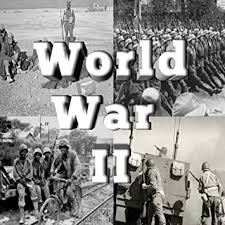
\includegraphics[scale=0.5]{ww2_01}
    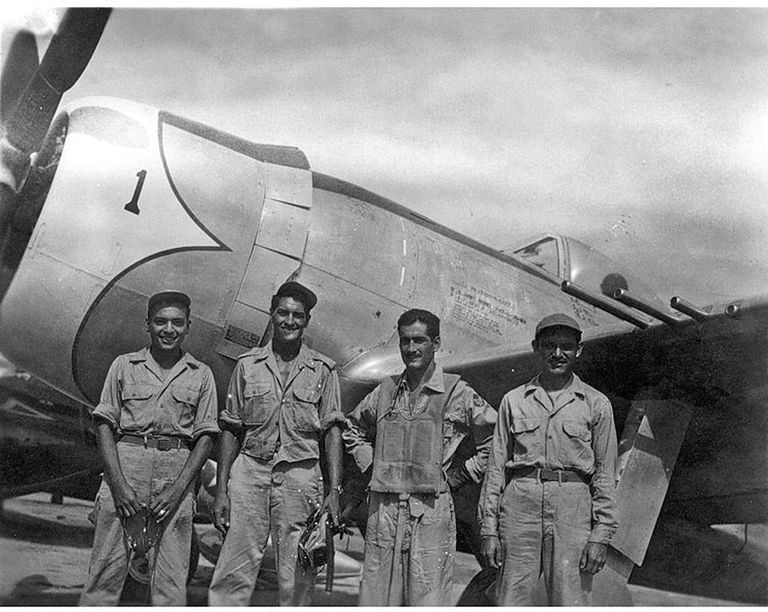
\includegraphics[scale=0.2]{ww2_02}
  \par}
\end{frame}

\begin{frame}{Desarrollo de la Investigación de Operaciones}
 \label{slide:or-dates}
  \begin{itemize} \justifying \parskip3mm
  \item<only@1> 1855. \href{https://en.wikipedia.org/wiki/Frederick_Winslow_Taylor}{Frederick W. Taylor}
  \item<only@1> 1884.  \href{https://en.wikipedia.org/wiki/Henry_Gantt}{Henry Gantt}
  \item<only@1> 1915. \href{https://en.wikipedia.org/wiki/Ford_Whitman_Harris}{Ford Whitman Harris}
  \item<only@1> 1917. \href{https://en.wikipedia.org/wiki/Agner_Krarup_Erlang}{A.K. Erlang}
  \item<only@1> 1930. \href{https://en.wikipedia.org/wiki/Horace_Clifford_Levinson}{Horace Clifford Levinson}
  \item<only@2> 1940. \href{https://www.informs.org/Explore/History-of-O.R.-Excellence/Biographical-Profiles/Blackett-Patrick-M.-S}{Patrick Maynard Stuart Blackett}  
    \item<only@2> 1947. \href{https://en.wikipedia.org/wiki/George_Dantzig}{George Dantzig}
    \item<only@2> 1950. \href{https://en.wikipedia.org/wiki/Ralph_E._Gomory}{Ralph E. Gomory}
  \item<only@2> \href{https://www.youtube.com/watch?v=ILWbaWrjgU4}{Historia de la IO} 
  \end{itemize}
\end{frame}


\begin{frame}{Características de la I.O.}
  \begin{enumerate} \justifying \parskip3mm
  \item Orientada a Sistemas
  \item Equipos interdisciplinarios
  \item Método Científico
  \item Nuevos Problemas
  \item Mejorar la calidad de las decisiones
  \item Tecnología
  \item Soluciones cuantitativas
  \item Factor humano
  \end{enumerate}
\end{frame}

\begin{frame}{Método Científico}
  \begin{enumerate} \justifying \parskip3mm
  \item Juicio
  \item Investigación
  \item Acción
  \end{enumerate}

  {\centering
      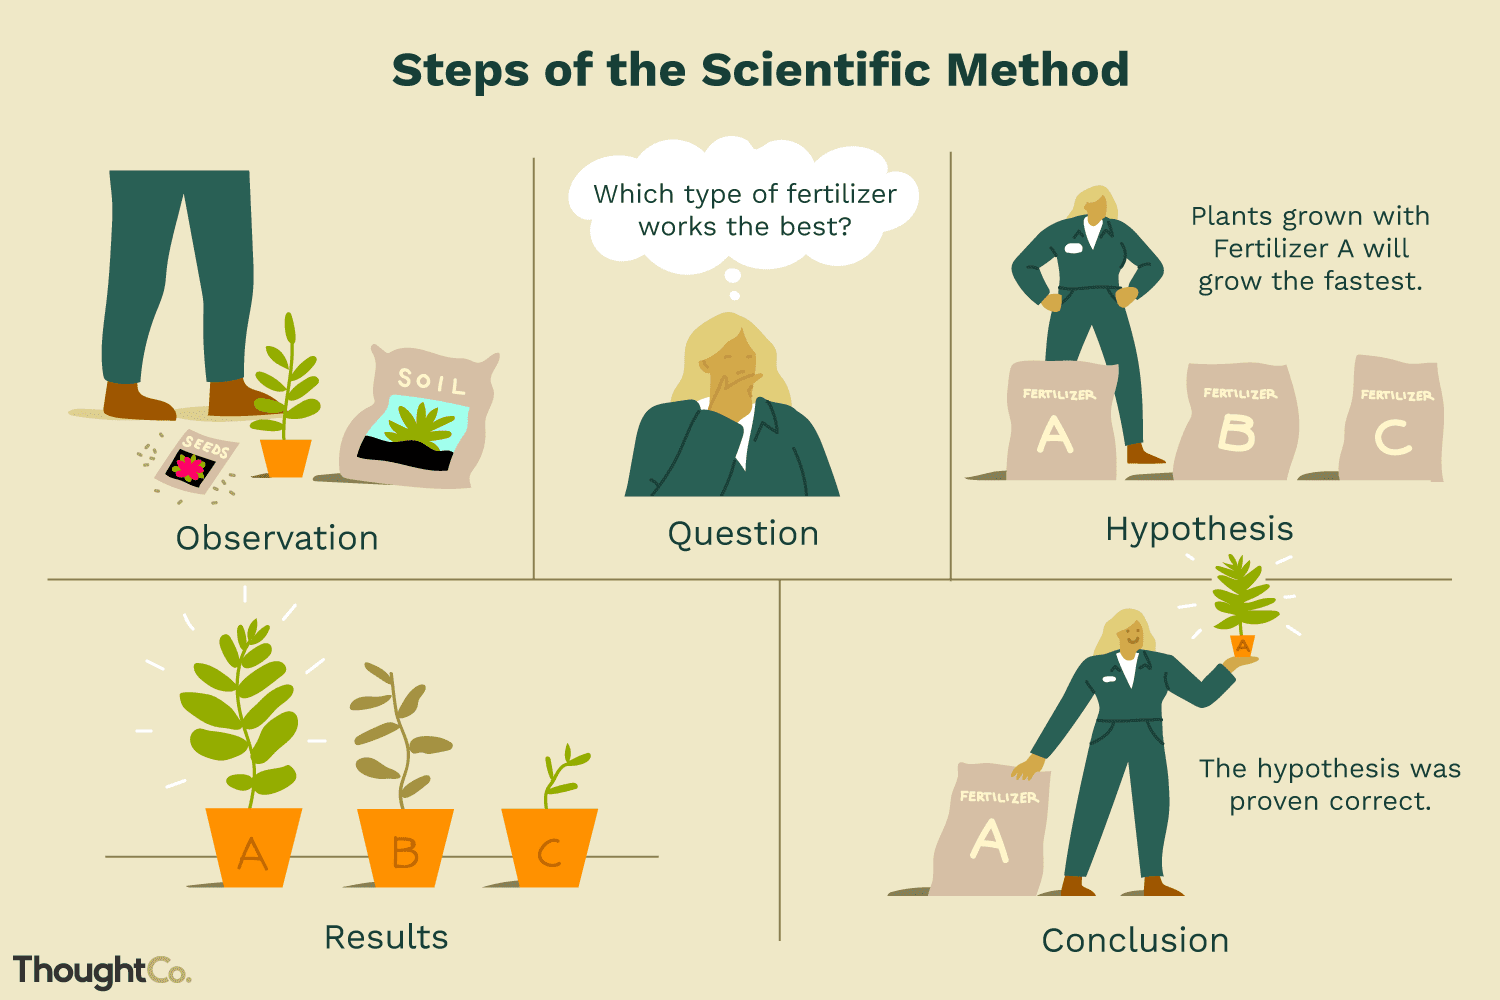
\includegraphics[scale=0.15]{scientific-method}
  \par}
\end{frame}

\begin{frame}{I.O. en Administración}
  \begin{columns}
    \column{0.5\textwidth}
\begin{itemize} \justifying \parskip3mm
  \item<only@1> Distribución
  \item<only@1> Planeación de la producción
  \item<only@1> Adquisiciones
  \item<only@1> Marketing
  \item<only@1> Finanzas
  \item<only@1> Investigación y Desarrollo
  \item<only@2>  Flujo de Efectivo
  \item<only@2> Control de Inventarios
  \item<only@2> Simulación
  \item<only@2> Presupuesto  
  \end{itemize}
  
  \column{0.5\textwidth}
  {\centering
    \includegraphics<1>[scale=0.5]{factory}
    \includegraphics<1>[scale=0.5]{logistics}
        \includegraphics<2>[scale=0.4]{logistics02}
  \par}
  \end{columns}
\end{frame}


\begin{frame}{Técnicas de I.O.}
  
  \begin{columns}
    \column{0.5\textwidth}
    \begin{enumerate} \justifying \parskip2mm
\item Programación Lineal.
\item Programación Dinámica.
\item Control de Inventarios.
\item Líneas de Espera.
\item Teoría de la Decisión.
\item Redes. CPM y PERT
\item Simulación.
\item Reemplazo
\end{enumerate}

\column{0.5\textwidth}
{\centering
  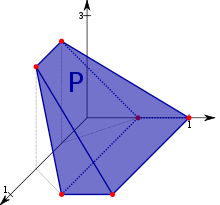
\includegraphics[scale=0.5]{polythope}
  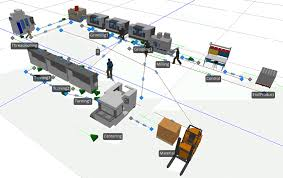
\includegraphics[scale=0.5]{simulation}
\par}
  \end{columns}
\end{frame}

\begin{frame}{Metodología}
  \begin{enumerate} \justifying \parskip3mm
  \item Formulación del Problema.
  \item Construcción del modelo.
  \item Solución.
  \item Verificación, validación. 
  \item Análisis de sensibilidad.
  \item Implementación.
  \end{enumerate}
\end{frame}


\begin{frameact}{Importancia de la  I.O.}
  En un documento Word o Google Docs escribe lo que se pide a continuación:

  \begin{itemize} \justifying  \parskip3mm
  \item Menciona en párrafos de 4 líneas como máximo las aportaciones que realizaron a la Investigación de Operaciones los siguientes científicos Blackett, Dantzig y Gomory. Usar un párrafo para cada personaje.   \hyperlink{slide:or-dates}{Dar click aquí}  para ver los links de cada biografía. % \href{https://www.youtube.com/watch?v=jg5IQ5Hf2G0}{Patrick Blackett. Draw my life (video)} que aparece en video del enlace.

  \item En tus propias palabras escribe una reflexión de máximo media cuartilla sobre el impacto que tiene la Investigación de Operaciones en nuestra vida a partir del video del \href{https://www.youtube.com/watch?v=sFWrmpXPVJw}{INFORMS Institute}
  \end{itemize}
\end{frameact}


%%% Local Variables:
%%% mode: latex
%%% TeX-master: "../slides"
%%% End:


\begin{frameact}{FedEx}
  Lea el artículo de referencia que describe todo el estudio de I.O. para FedEx. Enliste los diferentes beneficios financieros y no financieros que resultaron de este estudio. El artículo está disponible en el siguiente enlace: \href{https://drive.google.com/file/d/1b8VCLpjFeBWOssiuRRNjnjSkSGwoGaA9/view?usp=sharing}{“Absolutely, Positively Operations Research: The Federal Express Story”}
\end{frameact}


%%% Local Variables:
%%% mode: latex
%%% TeX-master: "../slides"
%%% End:


%%% Local Variables:
%%% mode: latex
%%% TeX-master: "slides"
%%% End:
